\documentclass[11pt]{article}
\usepackage[utf8]{inputenc}
\usepackage[T1]{fontenc}
\usepackage{amsmath}
\usepackage{amsfonts}
\usepackage{amssymb}
\usepackage[version=4]{mhchem}
\usepackage{stmaryrd}
\usepackage{multirow}
\usepackage{graphicx}
\usepackage[export]{adjustbox}
\graphicspath{ {./images/} }

\begin{document}
\section*{Reading}
Covariance, Correlation, Beta, and Autocorrelation

An important aspect of a return is the way that it correlates with other returns. This is because correlation affects diversification, and diversification drives the risk of a portfolio of assets relative to the risks of the portfolio's constituent assets. This section begins with an examination of covariance, then details the correlation coefficient. Much as standard deviation provides a more easily interpreted alternative to variance, the correlation coefficient provides a scaled and intuitive alternative to covariance. Finally, the section discusses the concepts of beta and autocorrelation.

\section*{Covariance}
The covariance of the return of two assets is a measure of the degree or tendency of two variables to move in relationship with each other. If two assets tend to move in the same direction, they are said to covary positively, and they will have a positive covariance. If the two assets tend to move in opposite directions, they are said to covary negatively, and they will have a negative covariance. Finally, if the two assets move independently of each other, their covariance will be zero. Thus, covariance is a statistical measure of the extent to which two variables move together. The formula for covariance is similar to that for variance, except that instead of squaring the deviations of one variable, such as the returns of fund $i$, the formula cross multiplies the contemporaneous deviations of two different variables, such as the returns of funds $i$ and $j$ :


\begin{equation*}
\text { Covariance }=\mathrm{E}\left[\left(R_{i}-\mu_{i}\right)\left(R_{j}-\mu_{j}\right)\right] \tag{1}
\end{equation*}


where $R_{\mathrm{i}}$ is the return of fund $i, \mu_{i}$ is the expected value or mean of $R_{i}, R_{j}$ is the return of fund $j$, and $\mu_{j}$ is the expected value or mean of $R_{j}$.

The covariance is the expected value of the product of the deviations of the returns of the two funds. Covariance can be estimated from a sample using Equation 2:


\begin{equation*}
\operatorname{Cov}\left(R_{i}, R_{i}\right)=\sigma_{i j}=\frac{1}{(T-1)} \sum_{t=1}^{T}\left[\left(R_{i t}-\bar{R}_{i}\right)\left(R_{j t}-\bar{R}_{j}\right)\right] \tag{2}
\end{equation*}


where $R_{i t}$ is the return of fund $i$ in time $t$, and $\bar{R}_{i}$ is the sample mean return of $R_{i t}$ and analogously for fund $j$. $T$ is the number of time periods observed.

The estimation of the covariance for a sample of returns from a market index fund and a real estate fund is shown in the exhibit, Covariance, Correlations, and Beta. Column 8 multiplies the fund's deviation from its mean return by the index's deviation from its mean return. Each of the products of the deviations is then summed and divided by $n-1$, where $n$ is the number of observations. The result is the estimated covariance between the returns over the sample period, shown near the

\begin{center}
\begin{tabular}{|c|c|c|c|c|c|c|c|c|}
\hline
 & \multirow[b]{2}{*}{(1) Month} & \multicolumn{3}{|c|}{Market Index} & \multicolumn{3}{|c|}{RE Fund} & \multirow[b]{2}{*}{(8) Cross} \\
\hline
 &  & (2) Return & (3) Deviation & (4) Dev2 & (5) Return & (6) Deviation & (7) Dev2 &  \\
\hline
 & 1 & -0.060 & -0.062 & 0.004 & -0.008 & -0.018 & 0.000 & 0.001 \\
\hline
 & 2 & -0.032 & -0.034 & 0.001 & -0.032 & -0.042 & 0.002 & 0.001 \\
\hline
 & 3 & -0.004 & -0.006 & 0.000 & 0.065 & 0.055 & 0.003 & 0.000 \\
\hline
 & . & . & . & . & . & . & . & . \\
\hline
 & . & . & . & . & . & . & . & . \\
\hline
 & . & . & . & . & . & . & . & . \\
\hline
 & 37 & 0.024 & 0.022 & 0.000 & 0.033 & 0.023 & 0.001 & 0.000 \\
\hline
 & 38 & 0.034 & 0.032 & 0.001 & 0.047 & 0.037 & 0.001 & 0.001 \\
\hline
 & 39 & 0.000 & -0.001 & 0.000 & -0.016 & -0.026 & 0.001 & 0.000 \\
\hline
 & 40 & 0.030 & 0.028 & 0.001 & 0.057 & 0.047 & 0.002 & 0.001 \\
\hline
 & Sum & 0.075 & 0.000 & 0.146 & 0.402 & 0.000 & 0.468 & 0.215 \\
\hline
 & Mean & 0.002 & 0.000 &  & 0.010 & 0.000 & 0.012 & 0.005 \\
\hline
 &  &  & Variance & $0.37 \%$ &  & Variance & $1.20 \%$ &  \\
\hline
Autocorrelation of market & 0.292 &  & Std. dev. & $6.11 \%$ &  & Std. dev. & $10.95 \%$ &  \\
\hline
Autocorrelation of fund & 0.142 &  &  &  &  & Cov. & 0.006 &  \\
\hline
Durbin-Watson of market & 1.393 &  &  &  &  & Cor. & 0.822 &  \\
\hline
Durbin-Watson of fund & 1.697 &  &  &  &  & Beta & 1.474 &  \\
\hline
\end{tabular}
\end{center}

bottom right-hand corner of the next exhibit.

Because covariance is based on the products of individual deviations and not squared deviations, its value can be positive, negative, or zero. When the return deviations are in the same direction, meaning they have the same sign, the cross product is positive; when the return deviations are in opposite directions, meaning they have different signs, the cross product is negative. When the cross products are summed, the resulting sum generates an indication of the overall tendency of the returns to move either in tandem or in opposition. Note that the table method illustrated in the Covariance, Correlations, and Beta exhibit simply provides a\\
format for solving the formula, which can be easily solved by software. Covariance is used directly in numerous applications, such as in the classic portfolio theory work of Markowitz.

\section*{Correlation Coefficient}
A statistic related to covariance is the correlation coefficient. The correlation coefficient (also called the Pearson correlation coefficient) measures the degree of association between two variables, but unlike the covariance, the correlation coefficient can be easily interpreted. The correlation coefficient takes the covariance and scales its value to be between +1 and -1 by dividing by the product of the standard deviations of the two variables. A correlation coefficient of -1 indicates that the two assets move in the exact opposite direction and in the same proportion, a result known as perfect linear negative correlation. A correlation coefficient of +1 indicates that the two assets move in the exact same direction and in the same proportion, a result known as perfect linear positive correlation. A correlation coefficient of zero indicates that there is no linear association between the returns of the two assets. Values between the two extremes of -1 and +1 indicate different degrees of association. Equation 3 provides the formula for the correlation coefficient based on the covariance and the standard deviations:


\begin{equation*}
\rho_{i j}=\sigma_{i j} /\left(\sigma_{i} \sigma_{j}\right) \tag{3}
\end{equation*}


where $\rho_{i j}$ (rho) is the notation for the correlation coefficient between the returns of asset $i$ and asset $j ; \sigma_{i j}$ is the covariance between the returns of asset $i$ and and $\sigma_{i}$ and $\sigma_{j}$ are the standard deviations of the returns of assets $i$ and $j$, respectively.

Thus, $\rho_{i j}$, the correlation coefficient, scales covariance, $\sigma_{i j}$, through division by the product of the standard deviations, $\sigma_{i} \sigma_{j}$. The correlation coefficient can therefore be solved by computing covariance and standard deviation as in the previous exhibit. and inserting the values into Equation 3. The result is shown in the Covariance, Correlations, and Beta exhibit.

\section*{The Spearman Rank Correlation Coefficient}
The Pearson correlation coefficient is not the only measure of correlation. There are some especially useful measures of correlation in alternative investments that are based on the ranked size of the variables rather than the absolute size of the variables. The returns within a sample for each asset are ranked from highest to lowest. The numerical ranks are then inserted into formulas that generate correlation coefficients that usually range between -1 and +1 . The Spearman rank correlation coefficient is a popular example.

The Spearman rank correlation is a correlation designed to adjust for outliers by measuring the relationship between variable ranks rather than variable values. The Spearman rank correlation for returns is computed using the ranks of returns of two assets. For example, consider two assets with returns over a time period of three years, illustrated here:

\begin{center}
\begin{tabular}{|c|c|c|}
\hline
Time Period & Return of Asset \#1 & Return of Asset \#2 \\
\hline
1 & $61 \%$ & $12 \%$ \\
\hline
2 & $-5 \%$ & $6 \%$ \\
\hline
3 & $0 \%$ & $4 \%$ \\
\hline
\end{tabular}
\end{center}

The first step is to replace the actual returns with the rank of each asset's return. The ranks are computed by first ranking the returns of each asset separately, from highest $(r a n k=1)$ to lowest ( $r a n k=3$ ), while keeping the returns arrayed according to their time periods:

\begin{center}
\begin{tabular}{|c|c|c|c|}
\hline
Time Period & Rank of Asset \#1 & Rank of Asset \#2 & Difference in Ranks $\left(d_{i}\right)$ \\
\hline
1 & 1 & 1 & 0 \\
\hline
2 & 3 & 2 & 1 \\
\hline
3 & 2 & 3 & -1 \\
\hline
\end{tabular}
\end{center}

This table demonstrates the computation of $d_{i}$, the difference in the two ranks associated with time period $i$. The Spearman rank correlation, $\rho_{s}$, can be computed using those differences in ranks and the total number of time periods, $n$ :

\begin{center}
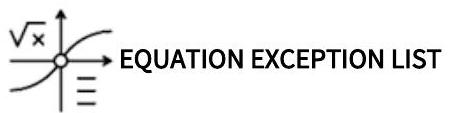
\includegraphics[max width=\textwidth]{2024_04_10_e3fefff2393dcb37755bg-3}
\end{center}

$$
\rho_{s}=1-\frac{6 \sum d_{i}^{2}}{n\left(n^{2}-1\right)}
$$

Using the data from the table, the numerator is 12 , the denominator is $3 \times 8=24$, and $\rho_{s}$ is 0.5 . Rank correlation is sometimes preferred because of the way it handles the effects of outliers (extremely high or low data values). For example, the enormous return of asset 1 in the previous table is an outlier, which will have a disproportionate effect on a correlation statistic. Extremely high or very negative values of one or both of the variables in a particular sample can cause the computed Pearson correlation coefficient to be very near +1 or -1 based, arguably, on the undue influence of the extreme observation on the computation, since deviations are squared as part of the computation. Some alternative investments have returns that are more likely to contain extreme outliers. By using ranks, the effects of outliers are lessened, and in some cases it can be argued that the resulting measure of the correlation using a sample is a better indicator of the true correlation that exists within the population. Note that the Spearman rank correlation coefficient would be the same for any return that would generate the same rankings. Thus, any return in time period 1 for the first asset greater than $0 \%$ would still be ranked 1 and would generate the same $\rho_{s}$.

\section*{The Correlation Coefficient and Diversification}
The correlation coefficient is often used to demonstrate one of the most fundamental concepts of portfolio theory: the reduction in risk found by combining assets that are not perfectly positively correlated. The next exhibit, Diversification between Two Assets illustrates the results of combining varying portions of assets A and B under three correlation conditions: perfect positive correlation, zero correlation, and perfect negative correlation.

\begin{center}
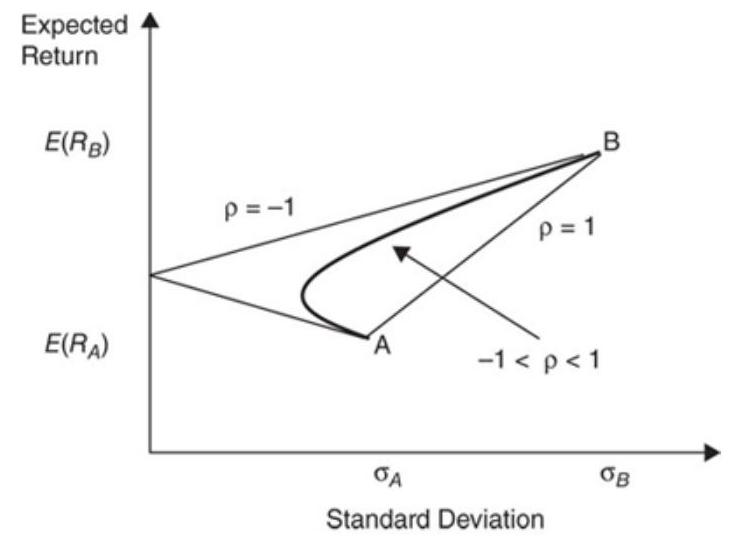
\includegraphics[max width=\textwidth]{2024_04_10_e3fefff2393dcb37755bg-4}
\end{center}

\section*{Diversification between Two Assets}
The highest possible correlation and least diversification potential is when the assets' correlation coefficient is +1: perfect positive correlation. The straight line to the lower right between points $A$ and $B$ in the above exhibit plots the possible standard deviations and mean returns achievable by combining asset $A$ and asset $B$ under perfect positive correlation. The line is straight, meaning that the portfolio risk is a weighted average of the individual risks. This illustrates that there are no benefits to diversification when perfectly correlated assets are combined. The idea is that diversification occurs when the risks of unusual returns of assets tend to cancel each other out. This does not happen in the case of perfect positive correlation, because the assets always move in the same direction and by the same proportion.

The greatest risk reduction occurs when the assets' correlation coefficient is -1: perfect negative correlation. The two upper-left line segments connecting points $A$ and $B$ in the above exhibit plot the possible standard deviations and mean returns that would be achieved by combining asset $A$ and asset $B$ under perfect negative correlation. Notice that the line between $\mathrm{A}$ and $\mathrm{B}$ moves directly to the vertical axis, the point at which the standard deviation is zero. This illustrates ultimate diversification, in which two assets always move in opposite directions; therefore, combining them into a portfolio results in rapid risk reduction, or even total risk reduction. This zero-risk portfolio illustrates the concept of a perfect two-asset hedge and occurs when the weight of the investment in asset $A$ is equal to the standard deviation of asset $B$ divided by the sums of the standard deviations of $A$ and $B$.

But the most realistic possibility is represented by the curve in the center of Diversification between Two Assets exhibit. This is the more common scenario, in which the assets are neither perfectly positively nor perfectly negatively correlated; rather, they have some degree of dependent movement. The key point to this middle line in the above exhibit is that when imperfectly correlated assets are combined into a portfolio, a portion of the portfolio's risk is diversified away. The risk that can be removed through diversification is called diversifiable, nonsystematic, unique, or idiosyncratic risk.

In alternative investments, the concept of correlation is central to the discussion of portfolio implications. Further, graphs with standard deviation on the horizontal axis and expected return on the vertical axis are used as a primary method of illustrating diversification benefits. Assets that generate diversification benefits are shown to shift the attainable combinations of risk and return toward the benefit of the investor, meaning less risk for the same amount of return. The key point is that imperfect correlation leads to diversification that bends portfolio risk to the left, representing the improved investment opportunities afforded by diversification.

In the case of asset returns, true future correlations can only be estimated. Past estimated correlation coefficients not only are subject to estimation error but also are typically estimates of a moving target, since true correlations should be expected to change through time, as fundamental economic relationships change. Further, correlation coefficients tend to increase (offer less diversification across investments and asset classes) in times of market stress, just when an investor needs diversification the most.

\section*{Beta}
The beta of an asset is defined as the covariance between the asset's returns and a return such as the market index, divided by the variance of the index's return, or, equivalently, as the correlation coefficient multiplied by the ratio of the asset volatility to market volatility:


\begin{equation*}
\beta_{i}=\operatorname{Cov}\left(R_{m}, R_{i}\right) / \operatorname{Var}\left(R_{m}\right)=\sigma_{i m} / \sigma_{m}^{2}=\rho_{i m} \sigma_{i} / \sigma_{m} \tag{5}
\end{equation*}


where $\beta_{i}$ is the beta of the returns of asset $i\left(R_{i}\right)$ with respect to a market index of returns, $R_{m}$. The numerator of the middle expression in Equation 5 measures the amount of risk that an individual stock brings into an already diversified portfolio. The denominator represents the total risk of the market portfolio. Beta therefore measures added systematic risk as a proportion of the risk of the index.

In the context of the capital asset pricing model (CAPM) and other single-factor market models, $R_{m}$ is the return of the market portfolio, and the beta indicates the responsiveness of asset $i$ to fluctuations in the value of the market portfolio. In the context of a single-factor benchmark, $R_{m}$ would be the return of the benchmark portfolio, and the beta would indicate the responsiveness of asset $i$ to fluctuations in the benchmark. In a multifactor asset pricing model, the beta indicates the responsiveness of asset $i$ to fluctuations in the given risk factor, as is discussed in the Financial Economics Foundations session.

The Covariance, Correlations, and Beta exhibit illustrates the computation of beta using a market index's return as a proxy for the market portfolio. Beta is similar to a correlation coefficient, but it is not bounded by +1 on the upside and -1 on the downside.

There are several important features of beta. First, it can be easily interpreted. The beta of an asset may be viewed as the percentage return response that an asset will have on average to a one-percentage-point movement in the related risk factor, such as the overall market. For example, if the market were to suddenly rise by\\
$1 \%$ in response to particular news, a fund with a market beta of 0.95 would be expected on average to rise $0.95 \%$, and a fund with a beta of 2.0 would be expected to rise $2 \%$. If the market falls $2 \%$, then a fund with a beta of 1.5 would have an expected decline of $3 \%$. But actual returns deviate from these expected returns due to any idiosyncratic risk. The risk-free asset has a beta of zero, and its return would therefore not be expected to change with movements in the overall market. The beta of the market portfolio is 1.0 .

The second feature of beta is that it is the slope coefficient in a linear regression of the returns of an asset (as the $Y$, or dependent variable) against the returns of the related index or market portfolio (as the $X$, or independent variable). Thus, the computation of beta in the Covariance, Correlations, and Beta exhibit using Equation 5 may be viewed as having identified the slope coefficient of the previously discussed linear regression. The session entitled Alpha, Beta, and Hypothesis Testing discusses linear regression.

Third, because beta is a linear measure, the beta of a portfolio is a weighted average of the betas of the constituent assets. This is true even though the total risk of a portfolio is not the weighted average of the total risk of the constituent assets. This is because beta reflects the correlation between an asset's return and the return of the market (or a specified risk factor) and because the correlation to the market does not diversify away as assets are combined into a portfolio.

Similar to the correlation coefficient between the returns of two assets, the beta between an asset and an index is estimated rather than observed. An estimate of beta formed with historical returns may differ substantially from an asset's true future beta for a couple of reasons. First, historical measures such as beta are estimated with error. Second, the beta of most assets should be expected to change through time as market values change and as fundamental economic relationships change. In fact, beta estimations based on historical data are often quite unreliable, although the most reasonable estimates of beta that are available may be based at least in part on historical betas.

\section*{Autocorrelation}
The autocorrelation of a time series of returns from an investment refers to the possible correlation of the returns with one another through time. For example, firstorder autocorrelation refers to the correlation between the return in time period $t$ and the return in the previous time period $(t-1)$. Positive first-order autocorrelation is when an above-average (below-average) return in time period $t-1$ tends to be followed by an above-average (below-average) return in time period $t$. Conversely, negative first-order autocorrelation is when an above-average (below-average) return in time period $t-1$ tends to be followed by a belowaverage (above-average) return in time period $t$. Zero autocorrelation indicates that the returns are linearly independent through time. Positive autocorrelation is seen in trending markets; negative autocorrelation is seen in markets with price reversal (i.e., mean reversion) tendencies.

We start here by assuming the simplest scenario: The returns on an investment are statistically independent through time, which means there is no autocorrelation. Further, we assume that the return distribution is stationary (i.e., the probability distribution of the return at each point in time is identical). Under these strict assumptions, the distribution of log returns over longer periods of time will tend toward being a normal distribution, even if the very short-term log returns are not normally distributed.

How do we know that log returns will be roughly normally distributed over reasonably long periods of time if the returns have no autocorrelation and if very-shortterm returns have a stationary distribution? One explanation is that the log return on any asset over a long time period such as a month is the sum of the log returns of the sub-periods. Even if the returns over extremely small units of time are not normally distributed, the central limit theorem indicates that the returns formed over longer periods of time by summing the independent returns of the sub-periods will tend toward being normally distributed.

Why might we think that returns would be uncorrelated through time? If a security trades in a highly transparent, competitive market with low transaction costs, the actions of arbitrageurs and other participants tend to remove pronounced patterns in security returns, such as autocorrelation. If this were not true, then arbitrageurs could make unlimited profits by recognizing and exploiting the patterns at the expense of other traders.

However, markets for securities have transaction costs and other barriers to arbitrage, such as restrictions on short selling. Especially in the case of alternative investments, arbitrage activity may not be sufficient to prevent nontrivial price patterns such as autocorrelation. The extent to which returns reflect nonzero autocorrelation is important because autocorrelation can affect the shape of return distributions. The following material discusses the relationships between the degree of autocorrelation and the shapes of long-period returns relative to short-period returns.

Autocorrelation of returns can be used as a general term to describe possible relationships or as a term to describe a specific correlation measure. Equation 6 describes autocorrelation in the context of a return series with constant mean:


\begin{equation*}
\text { Autocorrelation }=\mathrm{E}\left[\left(R_{t}-\mu\right)\left(R_{t-k}-\mu\right)\right] /\left(\sigma_{t} \sigma_{t-k}\right) \tag{6}
\end{equation*}


where $R_{t}$ is the return of the asset at time $t$ with mean $\mu$ and standard deviation $\sigma_{t}, R_{t-k}$ is the return of the asset at time $t-k$ with mean $\mu$ and standard deviation $\sigma_{t-k}$, and $k$ is the number of time periods between the two returns. Equation 6 is the same equation used to define the Pearson correlation coefficient in Equation 3 (with substitution of Equation 1 for covariance) except that Equation 6 specifies that the two returns are from the same asset and are separated by $k$ periods of time. Thus, autocorrelations, like correlation coefficients, range between -1 and +1 , with +1 representing perfect correlation.

There are unlimited combinations of autocorrelations that could theoretically be nonzero in a time series; thus, in practice, it is usually necessary to specify the time lags separating the correlations between variables. One of the simplest and most popular specifications of the autocorrelation of a time series is first-order autocorrelation. The first-order autocorrelation coefficient is the case of $k=1$ from Equation 6 , which is shown in Equation 7 :


\begin{equation*}
\text { First-Order Autocorrelation Coefficient }=\mathrm{E}\left[\left(R_{t}-\mu\right)\left(R_{t-1}-\mu\right)\right] /\left(\sigma_{t} \sigma_{t-1}\right) \tag{7}
\end{equation*}


Thus, first-order autocorrelation refers to the correlation between the return in time period $t$ and the return in the immediately previous time period, $t-1$. Note that in the case of first-order autocorrelation, the returns in time period $t-1$ would also be correlated with the returns in time period $t-2$; thus, the returns in time period $t$ would also generally be correlated with the returns in time period $t-2$, as well as those of earlier time periods. Because first-order autocorrelation is generally less than 1 , the idea is that the autocorrelation between returns diminishes as the time distance between them increases.

While autocorrelation would be zero in a perfectly efficient market, substantial autocorrelation in returns can occur when there is a lack of competition, when there are substantial transaction costs or other barriers to trade, or when there are returns that are calculated based on nonmarket values, such as appraisals. Autocorrelation of reported returns due to the use of appraised valuations or valuations based on the discretion of fund managers raises important issues, especially in the analysis of alternative investments.

Autocorrelation in returns has implications for the relationship between the standard deviations of a return series computed over different time lengths. Specifically, if autocorrelation is positive (i.e., returns are trending), then the standard deviation of returns over $T$ periods will be larger than the single-period standard deviation multiplied by the square root of $T$. If autocorrelation is zero, then the standard deviation of returns over $T$ periods will be equal to the single-period standard deviation multiplied by the square root of $T$. Finally, if autocorrelation is negative (i.e., returns are mean-reverting), then the standard deviation of returns over $T$ periods will be less than the single-period standard deviation multiplied by the square root of $T$.

An important task in the analysis of the returns of an investment is the search for autocorrelation. An informal approach to the analysis of the potential autocorrelation of a return series is through visual inspection of a scatter plot of $R_{t}$ against $R_{t-1}$. Positive autocorrelation causes more observations in the northeast and southwest quadrants of the scatter plot, where $R_{t}$ and $R_{t-1}$ share the same sign. Negative autocorrelation causes the southeast and northwest quadrants to have more observations, and zero autocorrelation causes balance among all four quadrants.

Another common approach when searching for autocorrelation is to estimate the first-order autocorrelation measure of Equation 7 directly, using sample data. The Covariance, Correlations, and Beta exhibit shows the estimated first-order autocorrelation coefficients for the two return series.

\section*{Higher-Order Autocorrelation and Partial Autocorrelation}
Analysis of alternative investments often involves consideration of whether a particular return series trends (i.e., has positive autocorrelation of returns) or meanreverts (has negative autocorrelation of returns). Substantial evidence indicates that the returns of some assets trend over some time intervals (e.g., monthly returns) and mean-revert over other time intervals (e.g., annual returns). The potential for returns to have positive and negative autocorrelation over different time horizons indicates that analysis of higher-order autocorrelations may be useful.

Equation 6 provides the formula for all orders or lags of autocorrelation. For example, in the case of second-order autocorrelation the equation specifies:

$$
\text { Second-Order Autocorrelation }=\mathrm{E}\left[\left(R_{t}-\mu\right)\left(R_{t-2}-\mu\right)\right] /\left(\sigma_{t} \sigma_{t-2}\right)
$$

Note, however, that the second-order autocorrelation between the returns in period $t$ and $t-2$ can be viewed as emanating both from the shared correlation of the two returns with the returns from period $t-1$ as well as potential correlation that is unique between periods $t$ and $t-2$. For example, suppose that a return series has a strong positive first-order autocorrelation coefficient of 0.7 . Even if there is no further causality of returns beyond one period, the second-order autocorrelation coefficient will be 0.49 , found as $0.7 \times 0.7$. In this example, an observed second-order autocorrelation coefficient statistically equal to 0.49 would be an indication that there is no further relation between returns $t$ and $t-2$. An observed second-order autocorrelation coefficient significantly greater than 0.49 would be an indication that there is additional positive relation between returns $t$ and $t-2$ beyond the correlation caused by the first-order correlation. Further, an observed second-order autocorrelation coefficient significantly less than 0.49 would be an indication that there is a negative second-order relation between returns $t$ and $t-2$ (apart from the positive correlation caused by the first-order correlation).

A partial autocorrelation coefficient adjusts autocorrelation coefficients to isolate the portion of the correlation in a time series attributable directly to a particular higher-order relation. Equation 8 depicts the formula for a second-order partial autocorrelation coefficient based on regular autocorrelation coefficients.


\begin{equation*}
\text { Second-Order Partial Autocorrelation Coefficient }=\left(\rho_{2}-\rho_{1}^{2}\right) /\left(1-\rho_{1}^{2}\right) \tag{8}
\end{equation*}


where $\rho_{i}$ is the ith-order autocorrelation coefficient as defined in Equation 6. Note that the numerator of Equation 8 "removes" the effect of first-order autocorrelation $\left(\rho_{1}^{2}\right)$ from the second-order autocorrelation $\left(\rho_{2}\right)$ to isolate the marginal effect of the period $t-2$ return on the return in period $t$.

To estimate partial autocorrelation coefficients for more than two periods, an analyst can use multiple regression with $R_{t}$ as the dependent variable and $R_{t-1}, R_{t-2}$, $R_{t-3}$, and so forth as independent variables. The regression coefficients are estimates of the partial autocorrelation coefficients. Multiple regression is discussed in Level II of the CAIA curriculum.

\section*{The Durbin-Watson Test for Autocorrelation}
A formal approach in searching for the presence of first-order autocorrelation in a time series is through the Durbin-Watson test. To test the hypothesis that there is no autocorrelation in a series involves calculating the Durbin-Watson statistic:

$$
\xrightarrow[\Xi]{\sqrt{x} \uparrow \text { EQUATION EXCEPTION LIST }}
$$

$$
D W=\frac{\sum_{t=2}^{T}\left(e_{t}-e_{t-1}\right)^{2}}{\sum_{t=1}^{T} e_{t}^{2}}
$$

where $e_{t}$ is the value in time period $t$ of the series being analyzed for autocorrelation. In alternative investments, the series being analyzed $\left(e_{t}\right)$ may be returns or a portion of returns, such as the estimated active return. A DWvalue of 2 indicates no significant autocorrelation (i.e., fails to reject the hypothesis of zero autocorrelation). If $D W$ is statistically greater than 2 , then the null hypothesis may be rejected in favor of negative autocorrelation; and if $D W$ is statistically less than 2 , then the null hypothesis may be rejected in favor of positive autocorrelation. The magnitude of the difference from 2 required to reject zero autocorrelation is complex, but a rule of thumb is that zero autocorrelation is rejected when $D W$ is greater than 3 , which is negative autocorrelation, or less than 1 , which is positive autocorrelation. The DW statistics for the market index and the real estate fund are reported in the bottom left-hand corner of the exhibit, Covariance, Correlations, and Beta. Note that the reported DW statistics for both of the return series fail to reject zero autocorrelation, even though the estimated autocorrelation coefficients appear quite positive.


\end{document}